\section{Biological Nanopores}

Biological nanopores are small perforations in a lipid bilayer, created
by a pore forming protein.  The majority of these proteins are toxins produced by
pathogenic bacteria. Their function in nature is to perforate the membrane of a cell,
causing cell depolarization and inducing an osmotic potential. These effects disrupt
vital cell functions or spill its nutrients into the environment, often times resulting
in the killing of the cell.

The reason scientists are interested in studying nanopores is related to their size.
These protein structures are generally only a few nanometres in diameter, making them
comparable in size to the tiny transistors found in modern computers.
Working at these small scales has the unavoidable complication, that it becomes difficult
to retrieve information from nano scale processes.
Developing sensors to probe this exotic length scale is thereby very relevant. This is
the exact problem nanopores provide a solution to, i.e. spectroscopy at the smallest
scale.

Before delving into ionic current spectroscopy, the primary application of these
nanopores, first a brief overview will be given of the structural properties of two
popular biological nanopores.

\subsection{$\alpha$-Hemolysin ($\alpha$-HL)}

The $\alpha$-Hemolysin ($\alpha$-HL) protein is the most commonly used pore forming
proteins to create biological nanopores. It is produced by the Staphylococcus aureus, a
bacterium commonly found in human microbiota.

The $\alpha$-HL pore(PDBID:...) is an oligomeric complex with multiple naturally
occurring variations. The most typical configuration
is a heptameric structure, meaning that there are seven protomers found in the complex.
The secondary structure elements consist principally of $\beta$-sheets, making it a
member
of the $\beta$-barrel pore-forming toxins. Through both electrostatic and hydrophobic
interactions, the $\alpha$-HL is bound to the membrane of a target cell. Here the
monomers assemble to a 'prepore' complex that transitions to the stable pore complex by
inserting the $\beta$-barrel into the membrane.

Structurally the shape of $\alpha$-HL resembles that of a hollow mushroom. The total
hight of the complex is 11nm and the maximum width is measured to be 10nm. The internal
chamber of the pore located at the cis side of the membrane is called the lumen.
The lumen of $\alpha$-HL is quite constricted measuring a diameter of 3nm. At the
membrane, the lumen chamber transitions into a protein stem, referred to as the
constriction of the pore further reducing the diameter of the chamber to a minimum of
1.5nm. Over the inside surface of  $\alpha$-HL the charges are relatively uniformly
distributed, which will play an important role in further applications.

%
% \begin{figure}[ht]
%   \begin{centering}
%   \adjustbox{minipage=1.3em,valign=t}{\subcaption{}\label{sfig:testa}}%
%   \begin{subfigure}[t]{\dimexpr.3\linewidth-1.3em\relax}
%   \centering
%   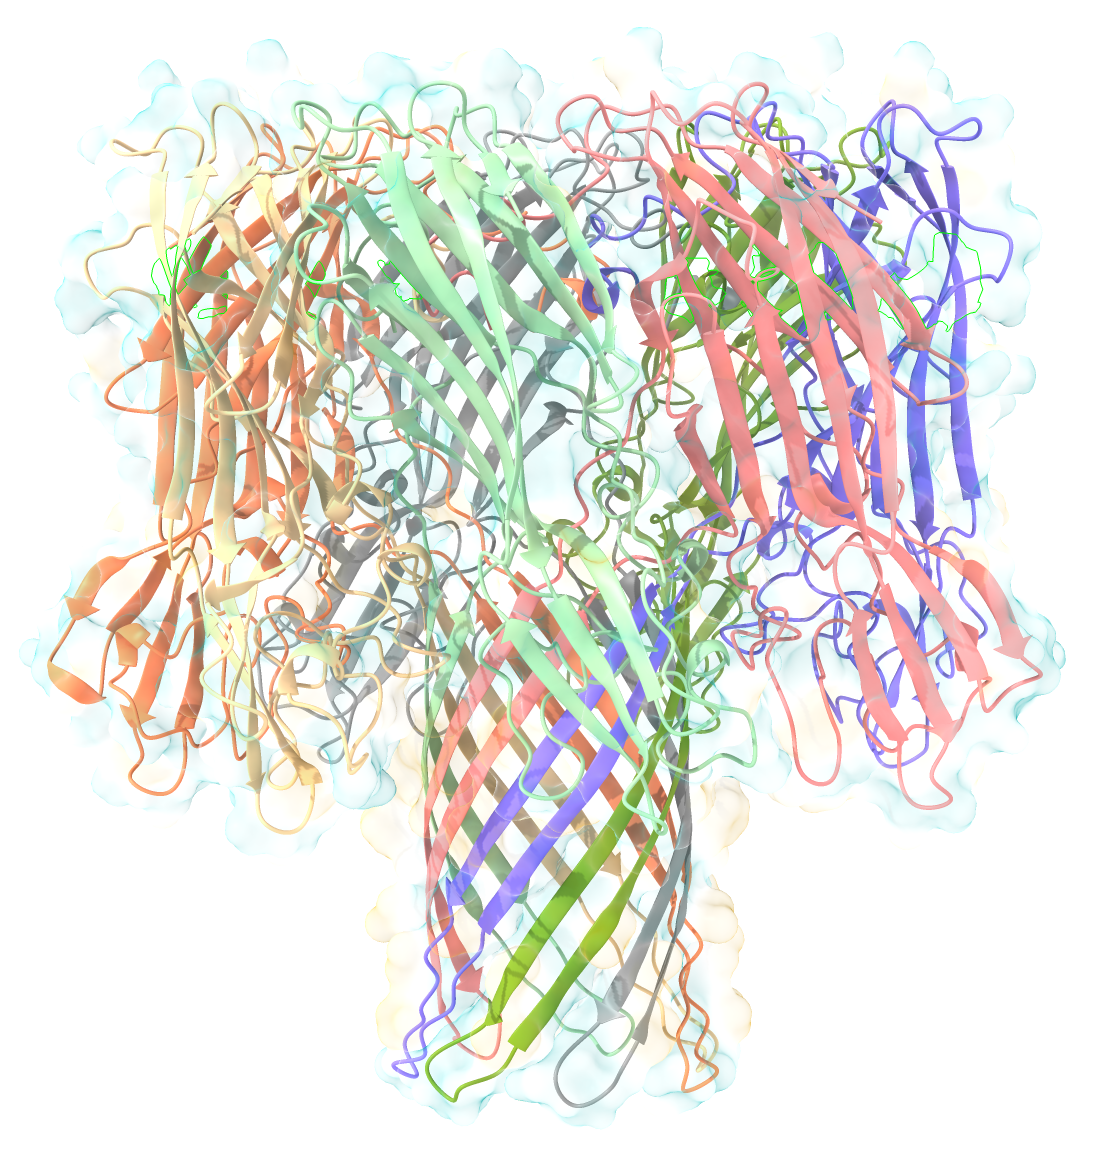
\includegraphics[width=\linewidth,valign=t]{Figures/ahl-front-s.png}
%   \end{subfigure}%
%   \adjustbox{minipage=1.3em,valign=t}{\subcaption{}\label{sfig:testa}}%
%   \begin{subfigure}[t]{\dimexpr.3\linewidth-1.3em\relax}
%   \centering
%   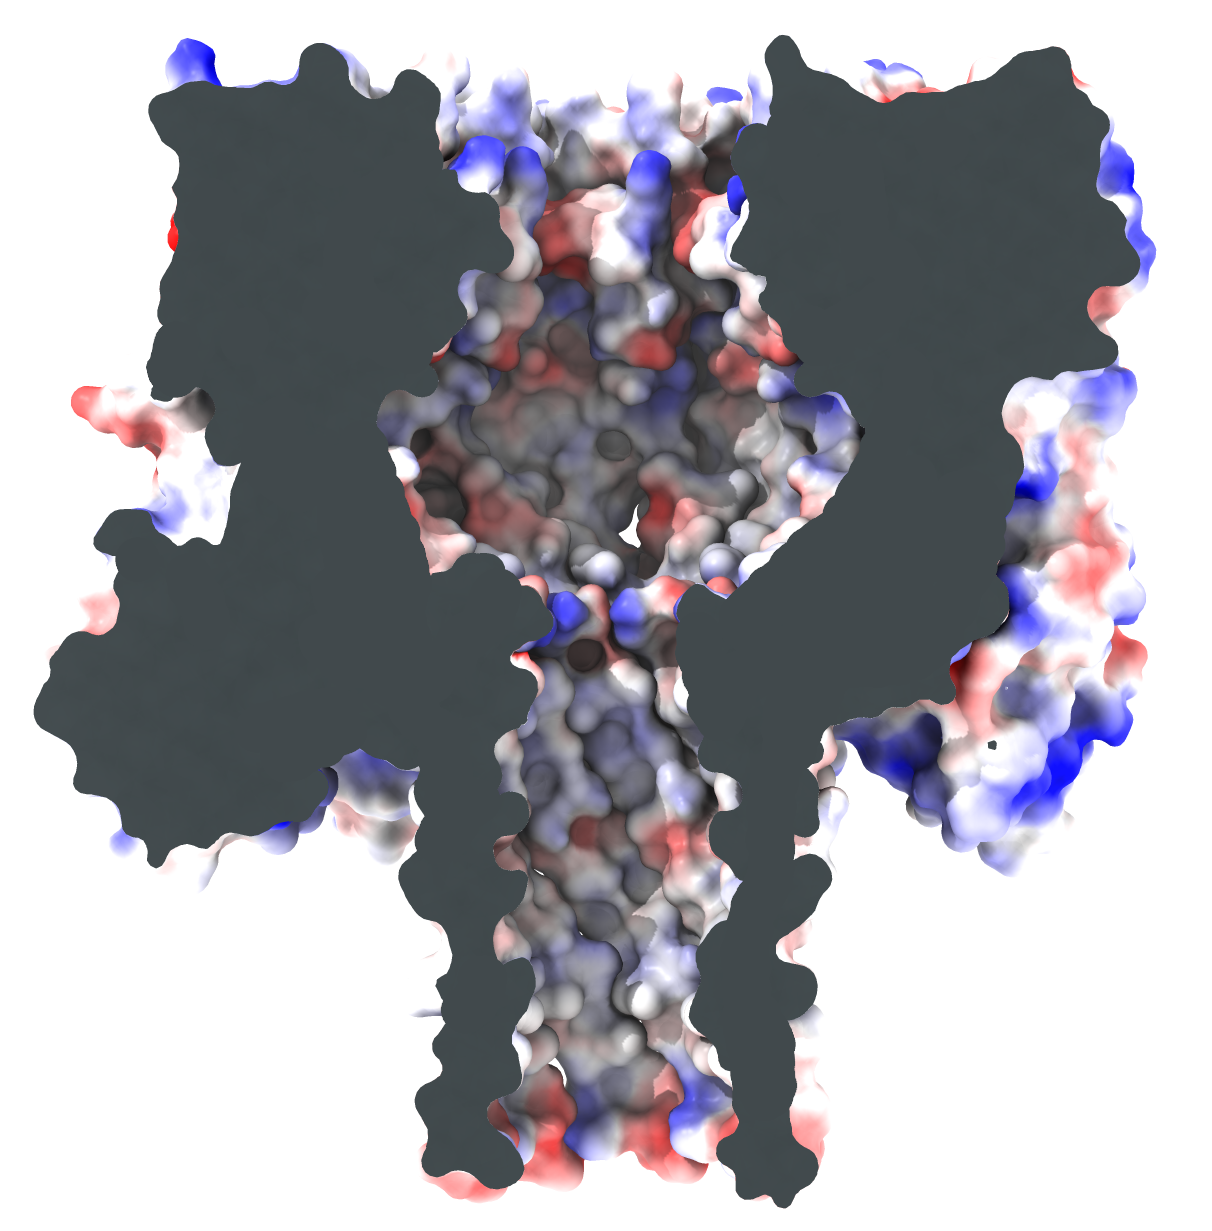
\includegraphics[width=\linewidth,valign=t]{Figures/ahl-elec.png}
%   \end{subfigure}%
%
%   \vspace{1.cm}
%
%   \adjustbox{minipage=1.3em,valign=t}{\subcaption{}\label{sfig:testb}}%
%   \begin{subfigure}[t]{\dimexpr.3\linewidth-1.3em\relax}
%   \centering
%   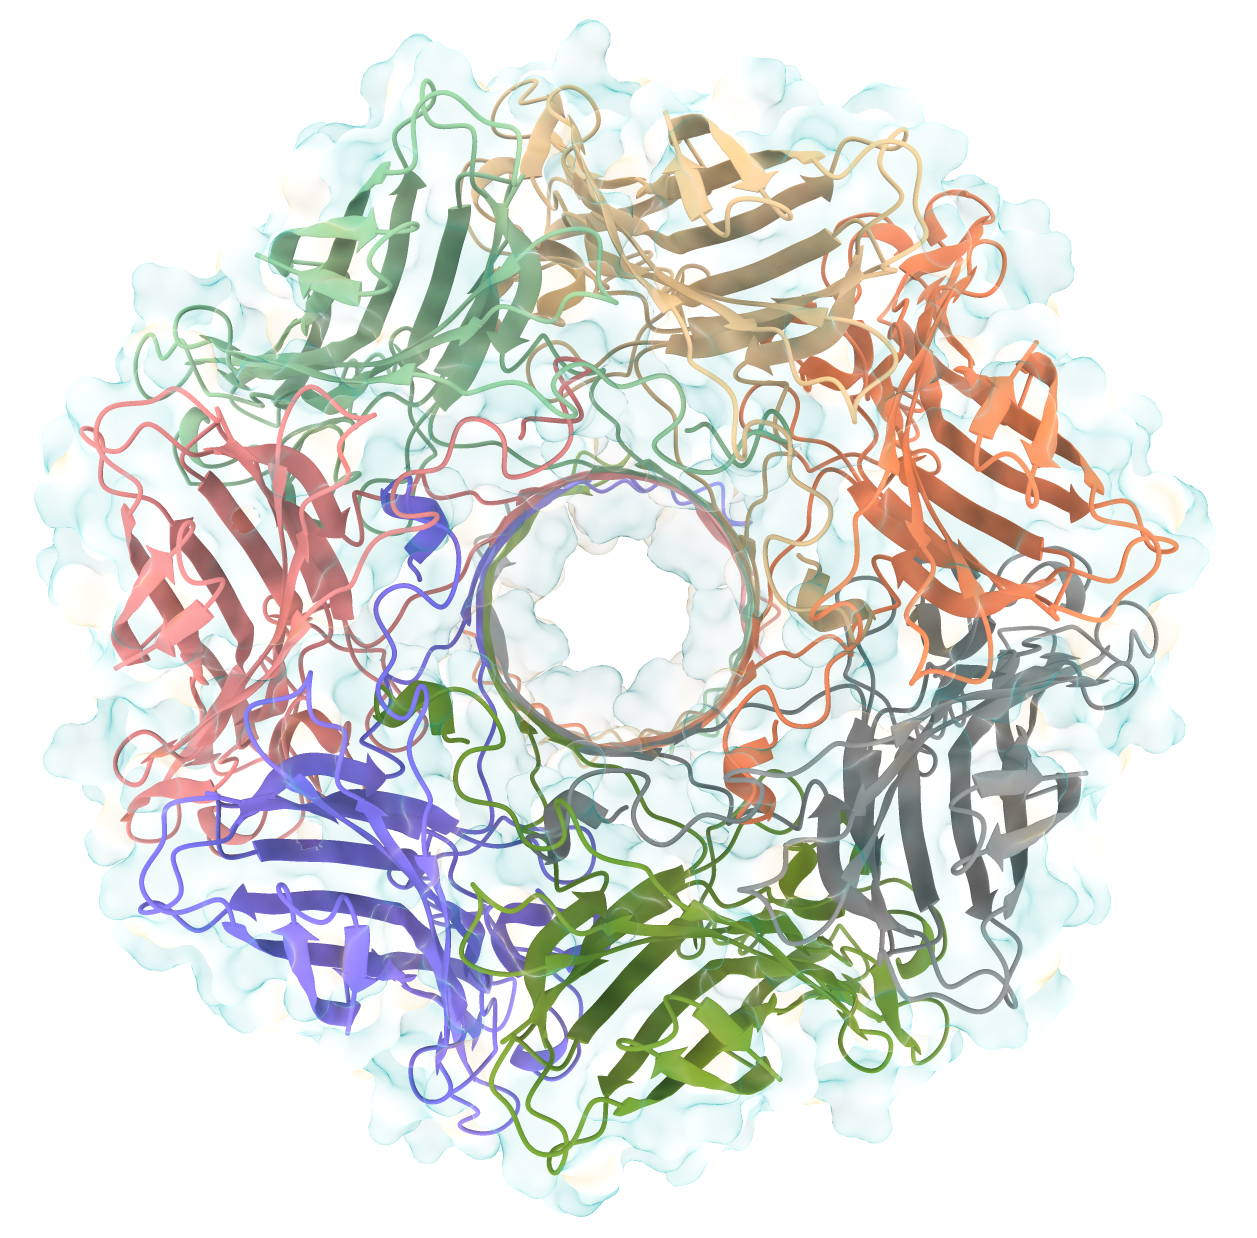
\includegraphics[width=\linewidth,valign=t]{Figures/ahl-top-s.png}
%   \end{subfigure}
%   \adjustbox{minipage=1.3em,valign=t}{\subcaption{}\label{sfig:testb}}%
%   \begin{subfigure}[t]{\dimexpr.3\linewidth-1.3em\relax}
%   \centering
%   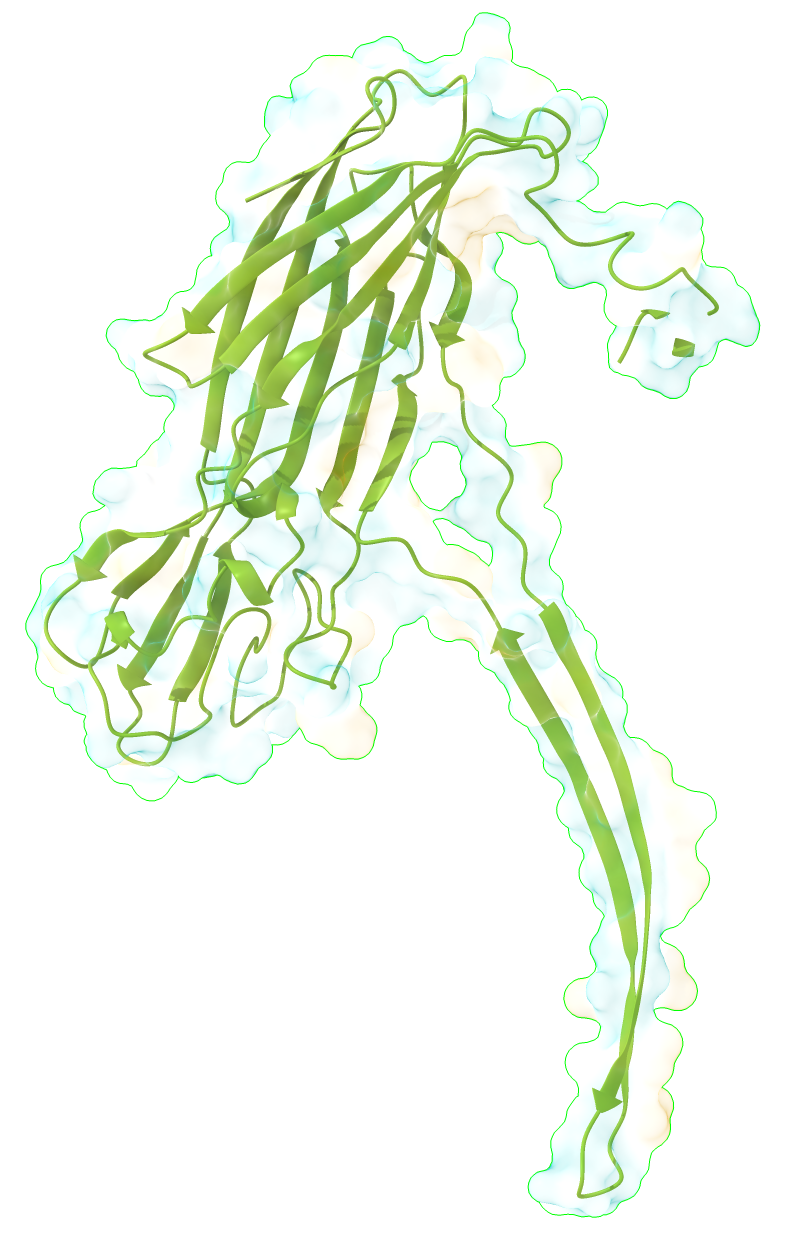
\includegraphics[width=\linewidth,valign=t]{Figures/ahl-mon-s.png}
%   \end{subfigure}
%
%   \caption{This is a figure}
%   \label{fig:test}
%   \end{centering}
% \end{figure}

\begin{figure}[ht]
  \begin{centering}
  \adjustbox{minipage=1.3em,valign=t}{\subcaption{}\label{sfig:testa}}%
  \begin{subfigure}[t]{\dimexpr.3\linewidth-1.3em\relax}
  \centering
  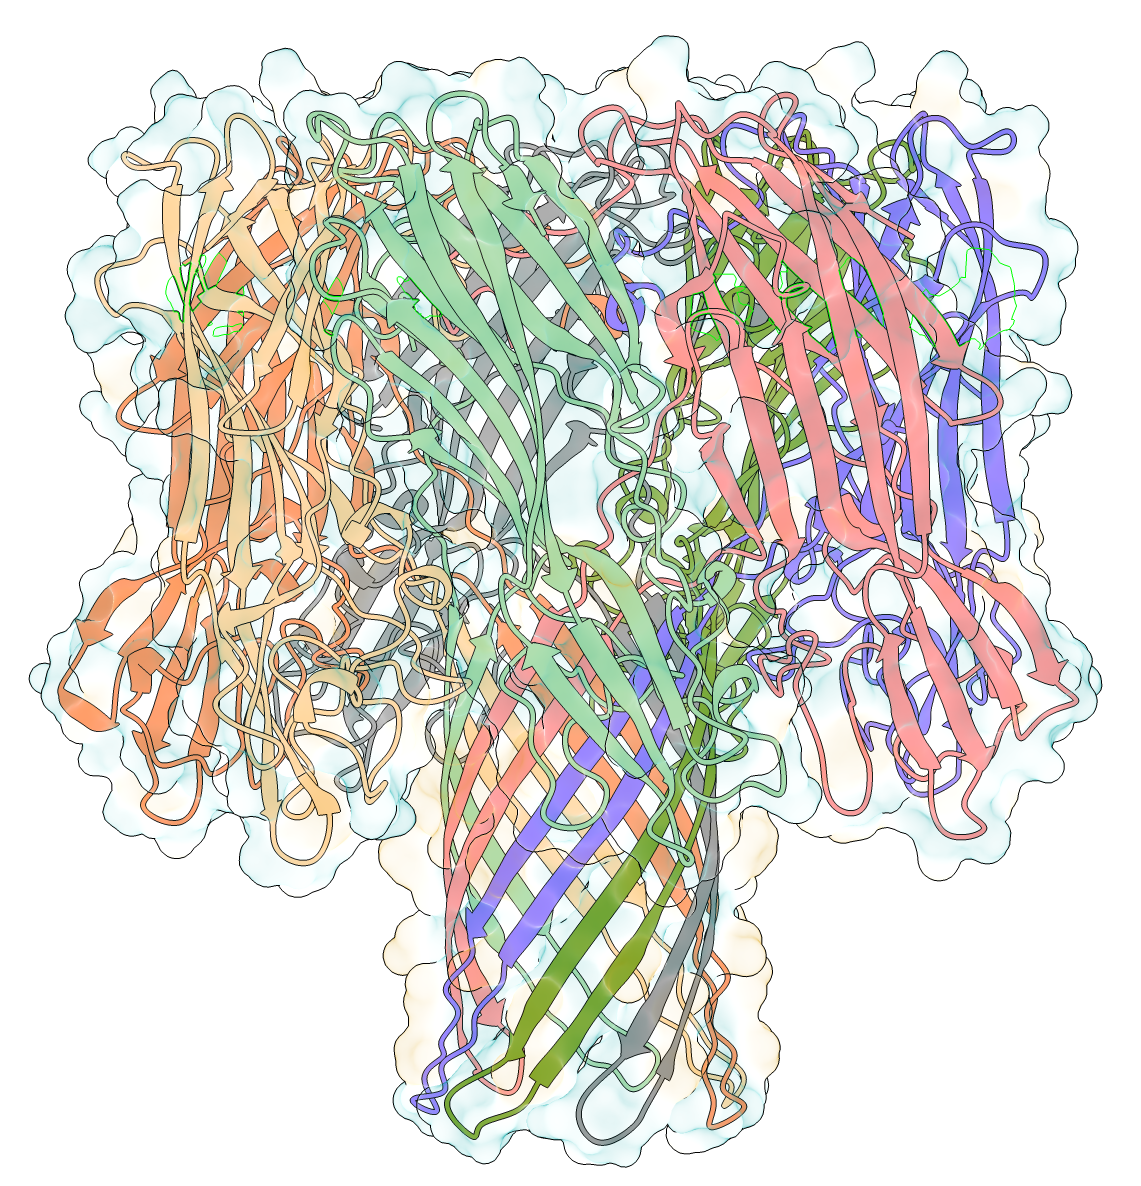
\includegraphics[width=\linewidth,valign=t]{Figures/ahl-front-c.png}
  \end{subfigure}%
  \adjustbox{minipage=1.3em,valign=t}{\subcaption{}\label{sfig:testb}}%
  \begin{subfigure}[t]{\dimexpr.3\linewidth-1.3em\relax}
  \centering
  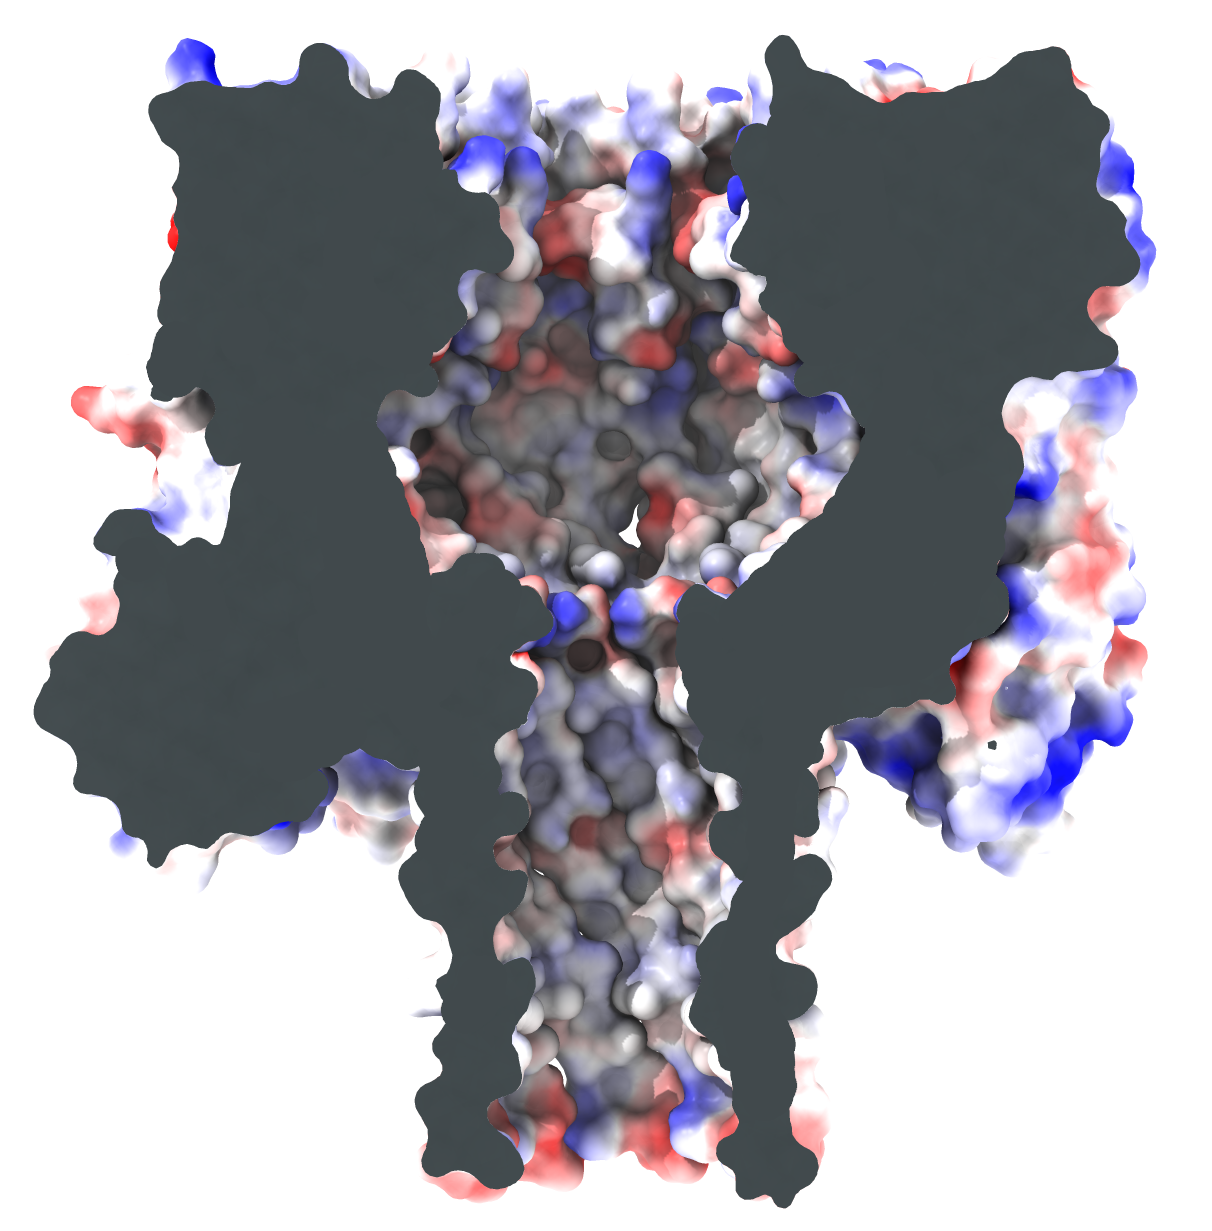
\includegraphics[width=\linewidth,valign=t]{Figures/ahl-elec.png}
  \end{subfigure}%

  \vspace{1.cm}

  \adjustbox{minipage=1.3em,valign=t}{\subcaption{}\label{sfig:testc}}%
  \begin{subfigure}[t]{\dimexpr.3\linewidth-1.3em\relax}
  \centering
  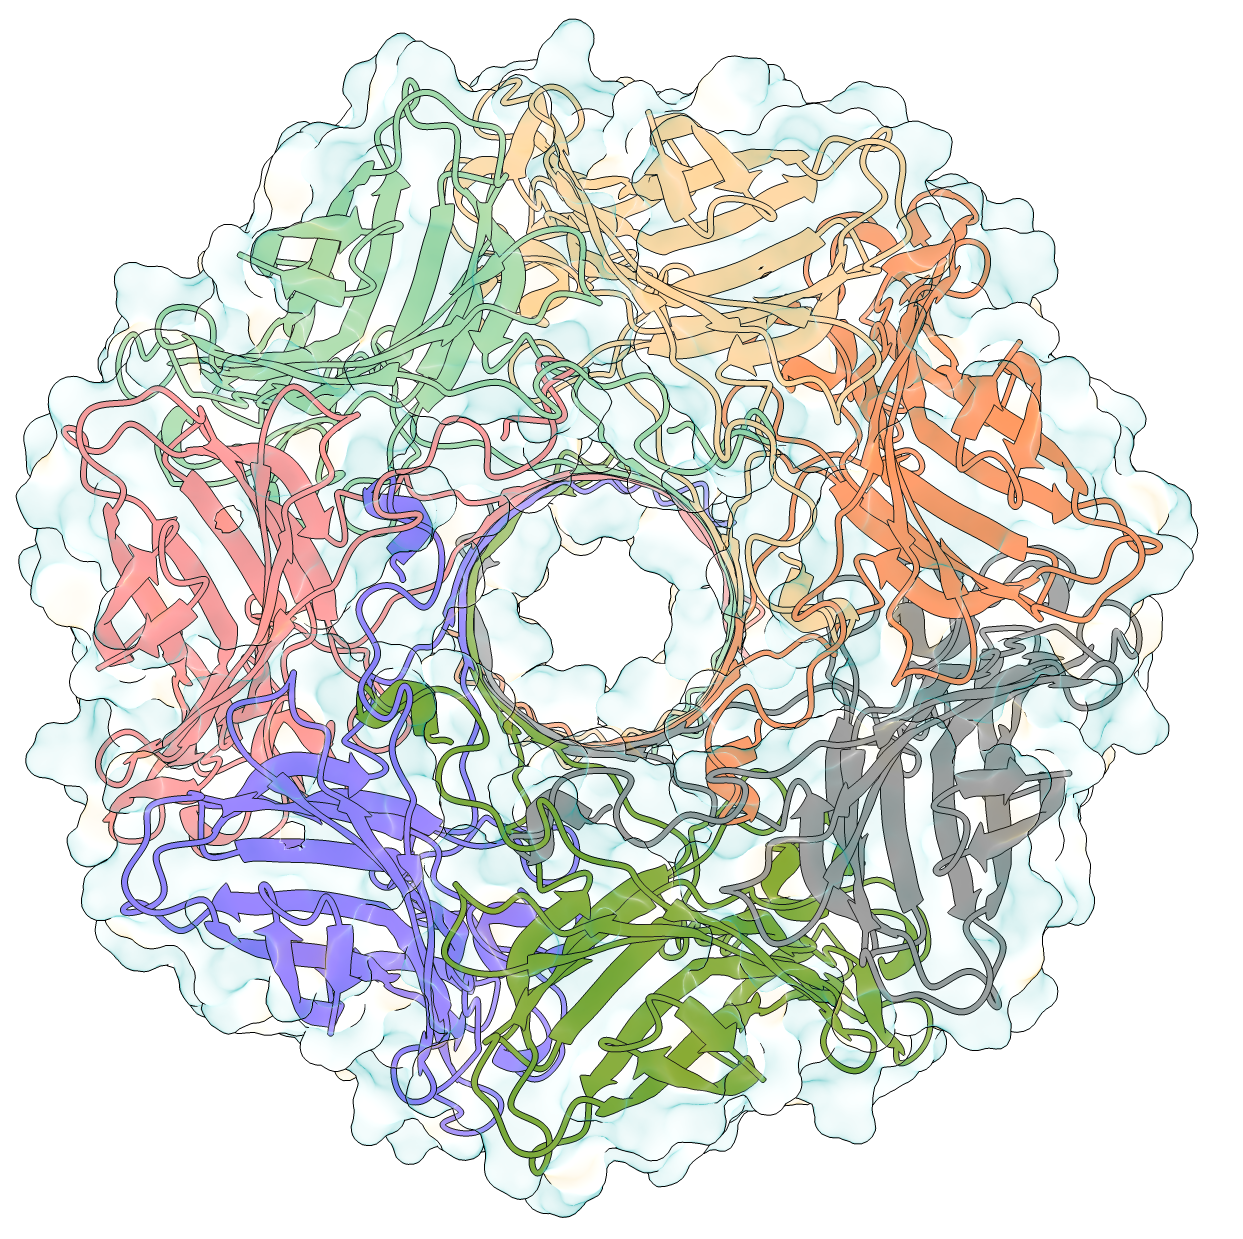
\includegraphics[width=\linewidth,valign=t]{Figures/ahl-top-c.png}
  \end{subfigure}
  \adjustbox{minipage=1.3em,valign=t}{\subcaption{}\label{sfig:testd}}%
  \begin{subfigure}[t]{\dimexpr.3\linewidth-1.3em\relax}
  \centering
  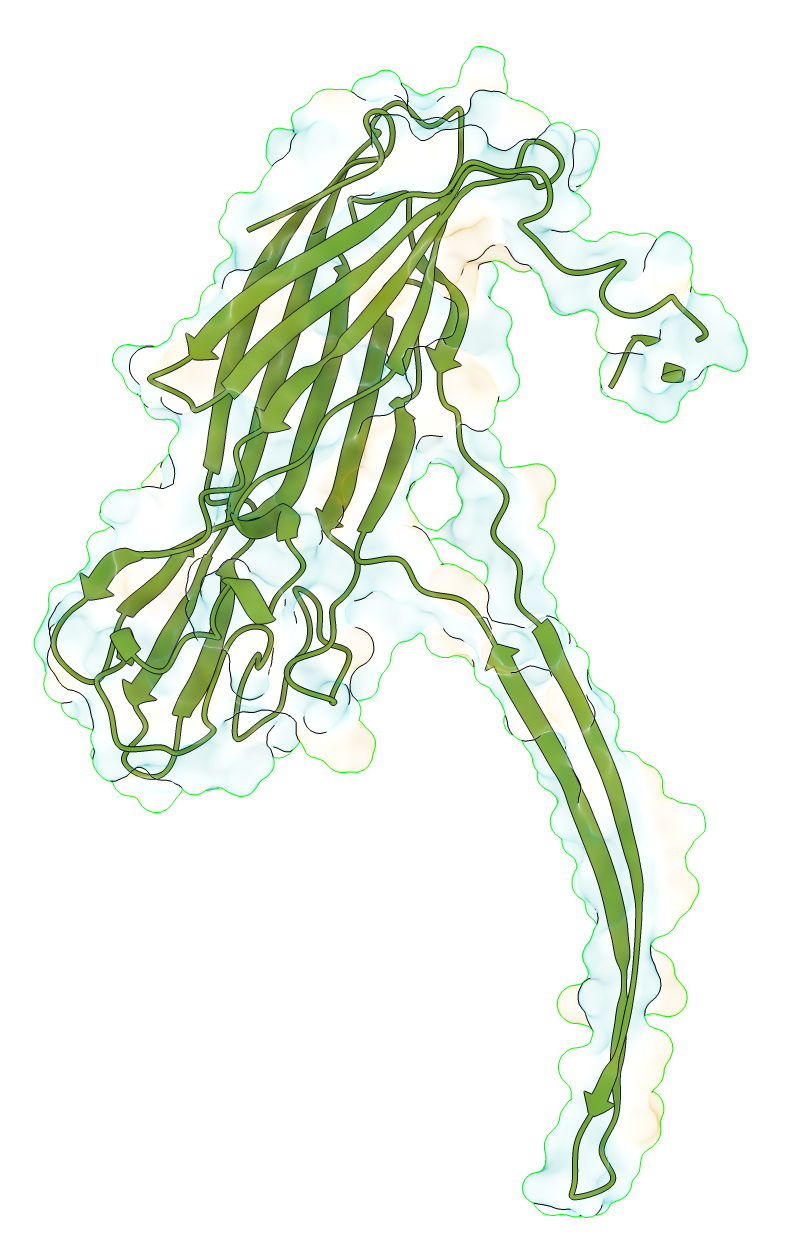
\includegraphics[width=.7\linewidth,valign=t]{Figures/ahl-mon-c.png}
  \end{subfigure}

  \caption{This is a figure}
  \label{fig:test}
  \end{centering}
\end{figure}



\subsection{Cytolysin A (ClyA)}

The Cytolysin A (ClyA) is a larger type of pore forming protein, first found to be
secreted by E. coli strains. The larger size of its lumen allows for different types of
applications, compared to smaller complexes like $\alpha$-HL. Most relevant for this
thesis, is the fact that the larger diameter of the pore's stem allows for translocation
of double stranded DNA.

The ClyA pore (PDBID:6MRT[cite]) is an oligomeric complex most typically found in a
 dodecameric configuration is, meaning that there are twelve protomers found in the
complex. In nature there are found small variations on this configuration. The secondary
structure elements consist principally of $\alpha$-helices, making it a member of the $
\alpha$-pore-forming toxins. The protein formation is induced by the hydrophobic
interactions between the $\beta$-hairpin and the solvent. The main structural
rearrangement in this process consists of swinging
out this $\beta$-tongue and inserting it into the membrane. After this transition, the
membrane-bounded monomers oligomerize to from the final pore structure.

Structurally the shape of ClyA resembles that of two hollow cylinders stacked on top of
each other. This cylinder approximation will be important later on in this thesis, where
it will be used to create a simplified model of the nanopore. The total hight of the
complex is
14nm and the maximum width is measured to be 11nm. The lumen's size of this nanopore
differentiates it from the previously discussed $\alpha$-HL. The cis entrance of the
lumen measures 6nm, while the constricted side of the pore is still 3.6nm in diameter. In
contrary to the $\alpha$-HL, the inside surface of ClyA has a net negative charge,
making it cation sensitive. This excess charge will induce an significant
 coulomb interaction between the pore and negatively charged analytes.

\begin{figure}[ht]
  \begin{centering}
  \adjustbox{minipage=1.3em,valign=t}{\subcaption{}\label{sfig:testa}}%
  \begin{subfigure}[t]{\dimexpr.3\linewidth-1.3em\relax}
  \centering
  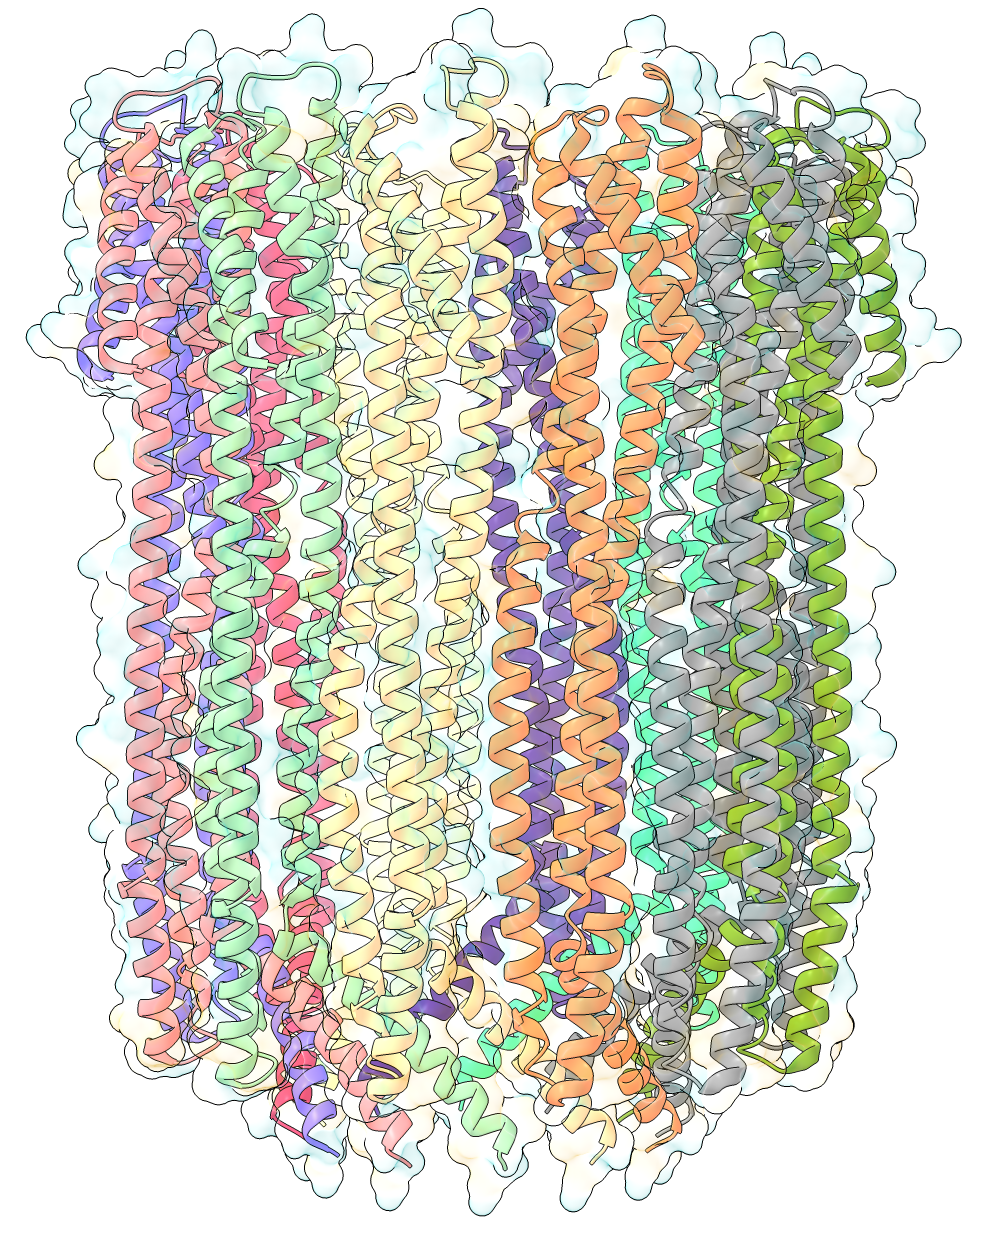
\includegraphics[width=\linewidth,valign=t]{Figures/clya-front-c.png}
  \end{subfigure}%
  \adjustbox{minipage=1.3em,valign=t}{\subcaption{}\label{sfig:testa}}%
  \begin{subfigure}[t]{\dimexpr.3\linewidth-1.3em\relax}
  \centering
  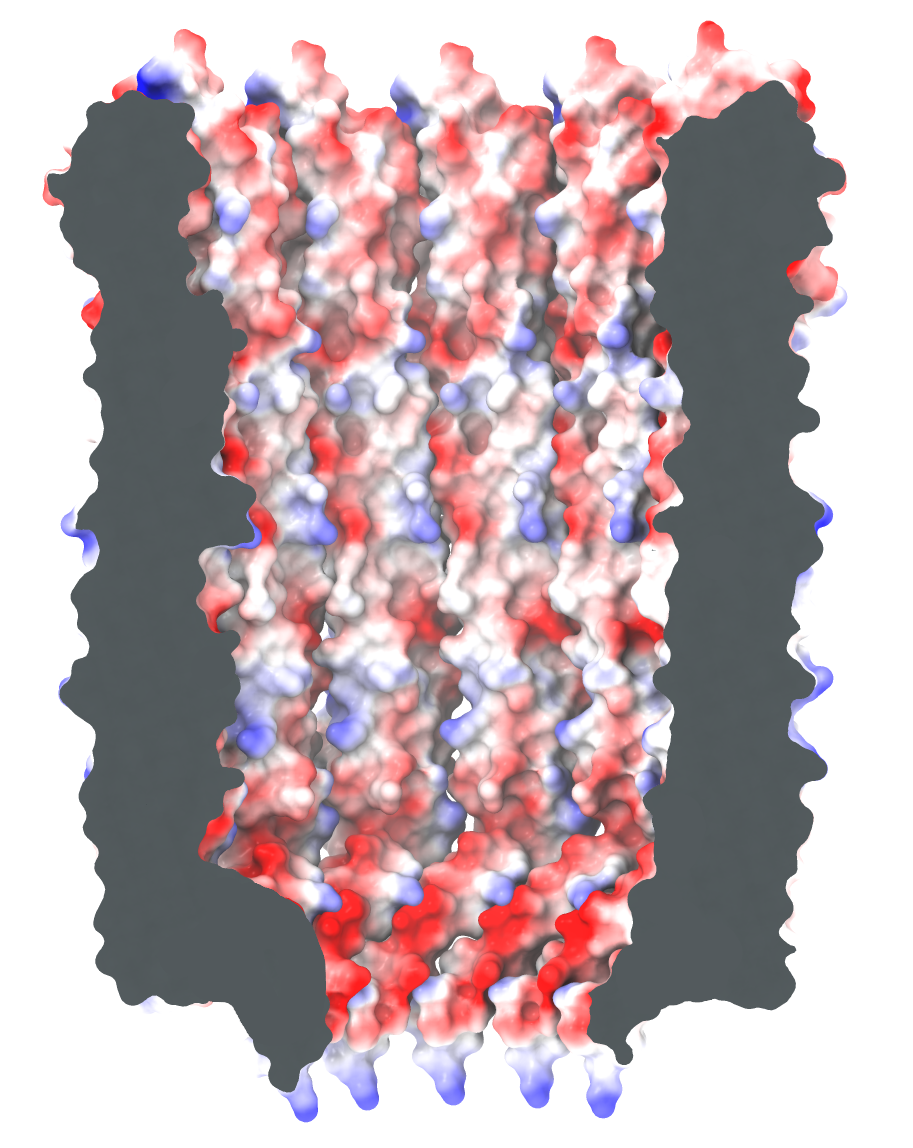
\includegraphics[width=\linewidth,valign=t]{Figures/clya-elec.png}
  \end{subfigure}%

  \vspace{1.cm}

  \adjustbox{minipage=1.3em,valign=t}{\subcaption{}\label{sfig:testb}}%
  \begin{subfigure}[t]{\dimexpr.3\linewidth-1.3em\relax}
  \centering
  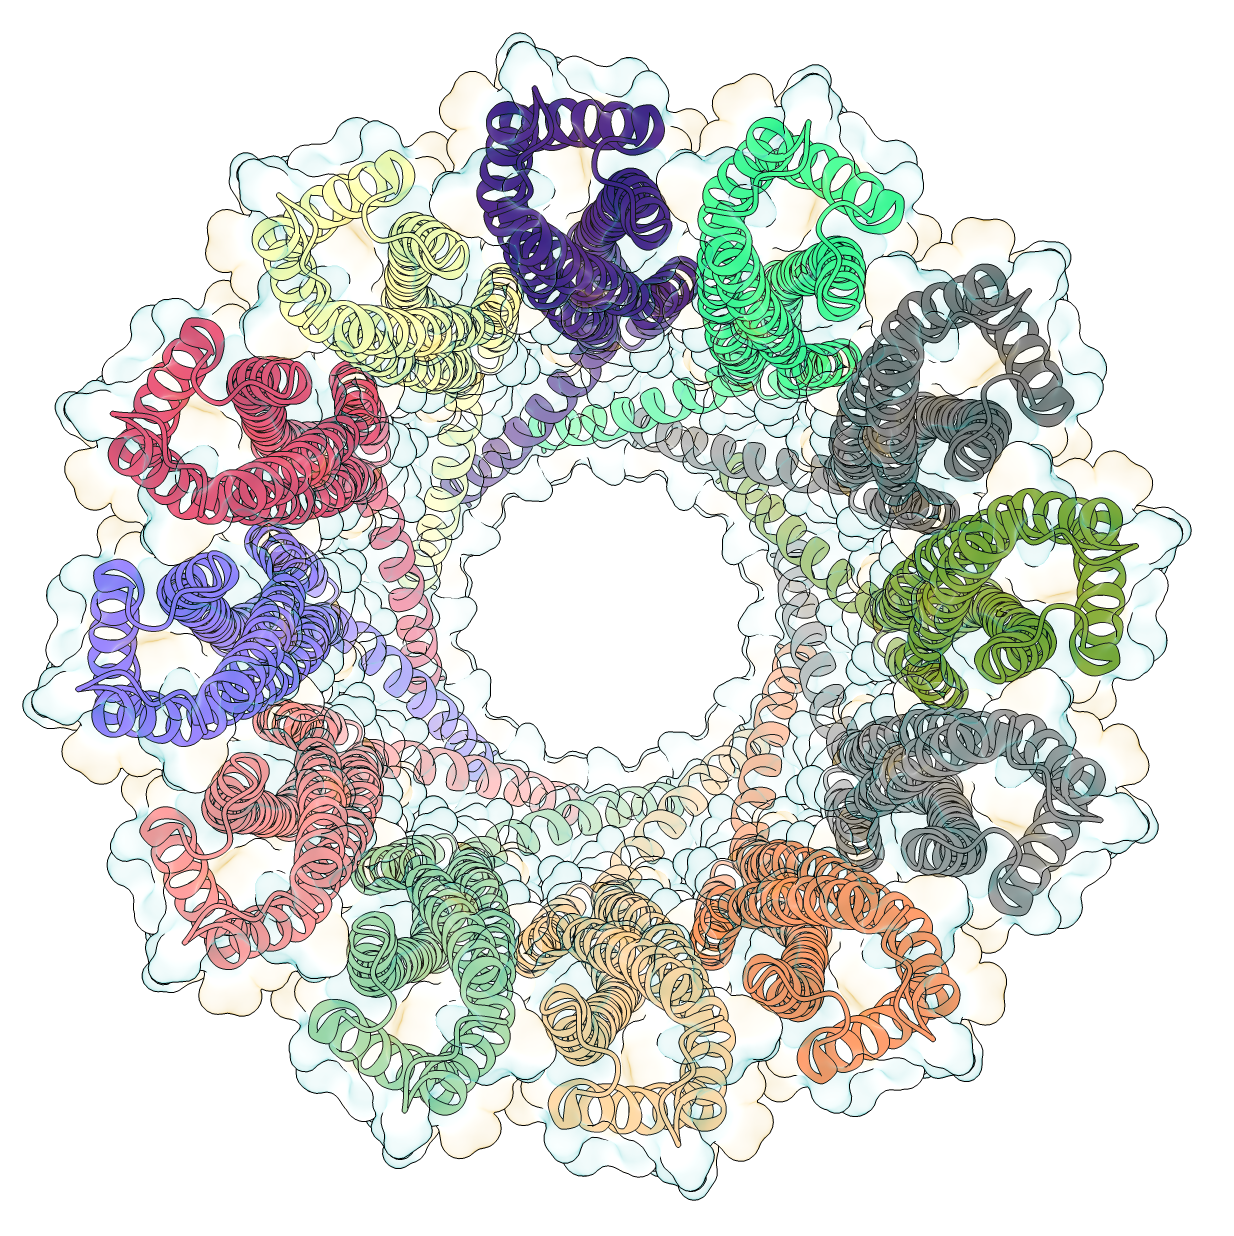
\includegraphics[width=\linewidth,valign=t]{Figures/clya-top-c.png}
  \end{subfigure}
  \adjustbox{minipage=1.3em,valign=t}{\subcaption{}\label{sfig:testb}}%
  \begin{subfigure}[t]{\dimexpr.3\linewidth-1.3em\relax}
  \centering
  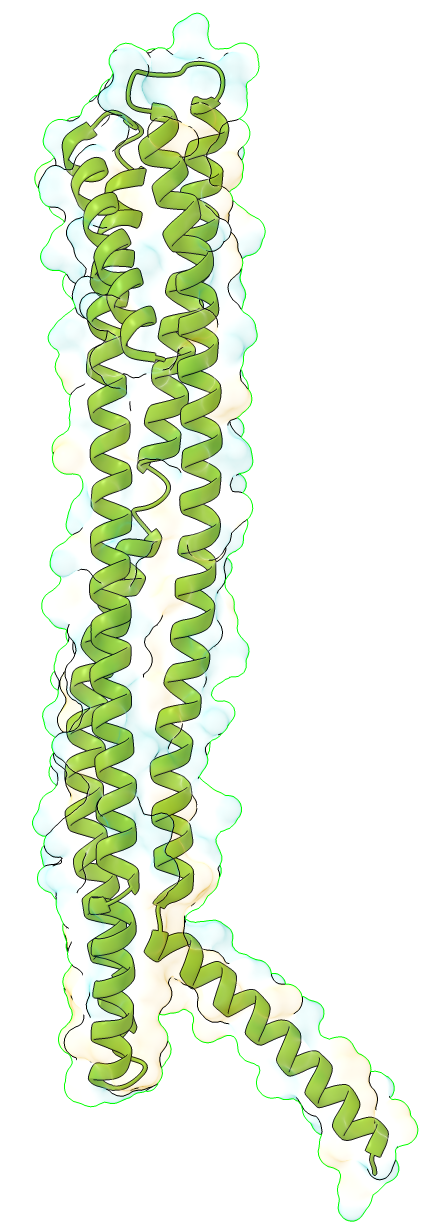
\includegraphics[width=.35\linewidth,valign=t]{Figures/clya-mon-c.png}
  \end{subfigure}

  \caption{This is a figure}
  \label{fig:test}
  \end{centering}
\end{figure}


\subsection{Ionic current spectroscopy}
In recent years the study of nanopores became a popular research domain, mainly
due to the development of the nanopore-based ionic current spectroscopy. For the case of
biological nanopores, this method depicted in figure ... A lipid bilayer is perforated
using a pore forming protein, for example $\alpha$-HL. The membrane separates two
compartments filled with a saline solution. When a potential difference is created
over the membrane, the nanopore mediates an ion current between the two liquid-filled
compartments.

This ion current through the pore can accurately be measured. If the pore is empty we
refer to the measured current as the open pore current.  However the applied electric
field also induces forces upon analytes dissolved in the liquid. The net result of these
interactions is a flux of analytes towards and in some cases through the nanopore.
Analytes located inside of the nanopore partially block the ion current through the pore,
reducing the measured current. Using machine learning algorithms, the time series of
these current fluctuation can be measured and identified with particular analytes in the
solution. These methods are so precise, that they allow for single cell spectroscopy.

It should be noted that besides these biological nanopores, there are also inorganic
nanopores under development. An example of inorganic nanopres are solid state nanopores,
created by making perforations in a semi-conductor wafer. While currently not as
accessible as biological nanopres, mainly due to their high production cost, this method
has some major advantages. First of all the material properties provide a chemical
robustness not present in biological nanopores. The production process also allows for
easy scalability and customisability. While currently not as widely used as biological
nanopores, due to their customisability and robustness, solid state nanopores will prove
to be an important asset in future nanotechnology.
